%!TEX root = ../Master.tex

\section{Software} 
\label{sec:software}

The software was written mostly in c++ for its speed, and partly in python for easy integration with an existing driver for the neato robot. ROS (Robot Operating System) was used for visualization and communication.

\subsection{ROS}
To be able to easily test and validate the implemented AI methods, we used ROS to visualize the system. ROS  is a collection of software for building robot systems and has a large collection of packages for 3D visualization, navigation, mapping, localization, planning, etc. Only the visualization and communication parts of ROS has been used in this project. This is chosen due to the purpose of trying to implement localization, planning, and control ourself. \\

A ROS project consists of a collection of processes with a single responsibility, i.e. planning, vision, control, etc. ROS also handles the communication between these processes. The processes are conceptualized as nodes in a network which can communicate by publishing and subscribing on topics. \\

The communication in ROS consists of messages with a specific data type. The data type could be anything from simple integers to LaserScans which describes a scan from a lidar and extra header information as a time stamp and a sequence number if the order of scans are important. A node can also contain services which can be called with a request-response communication model, instead of the the publish-subscribe model between nodes.\\

ROS master is the program that coordinates the communication between the nodes. It also works as a registry for nodes, services, topics, etc.

\subsubsection{ROS Nodes}
The system implements two ROS nodes, the first is a driver for the Neato robot and the second is the navigation system.\\

The driver is a modified version of an open source driver for the robot. \cite{neato} The open source driver implements an older version of the serial protocol for the Neato robot. This has been modified to implement the newer protocol which our robot uses.\\

The navigation node implements all of the AI algorithms; localization, planning and control. The two nodes communicate using ROS messages for lidar scans and control commands. 

\subsection{Neato driver node}
The neato driver node subscribes on the "command" topic to get the motion commands from the navigation node. After executing the motion command the node publishes the latest laser scan to the navigation node. This way the navigation node will always get a laser scan from the new position of the robot.

\subsection{Navigation node}
Most of the work has been in the navigation node where localization, planning and control is implemented. When a laser scan is received from the robot, a calculation of the next motion command is initialized. The Monte Carlo localizer is used to get an estimate of the current position. The uncertainty of the estimate is used to determine whether to trust it and follow a path to the goal or to keep driving around the map to decrease the uncertainty of the estimate. \autoref{fig:diagram} shows a class diagram for the navigation software. Each class is explained in more detail in the following sections.

\begin{figure}[H]
\centering
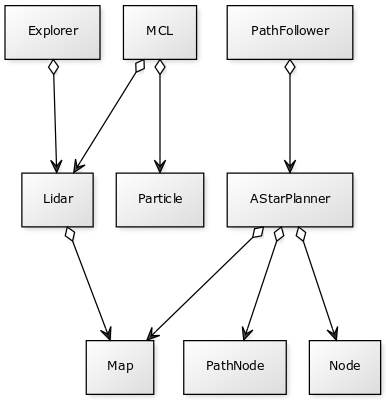
\includegraphics[scale=0.40]{images/diagram}
\caption{Class diagram for control and localization program}
\label{fig:diagram}
\end{figure}

\subsubsection{Map}
The map is implemented as a matrix of grid cells where each grid cell represents a $25cm\times25cm$ square in the real world. Each grid cell consists of an integer describing what is in the grid cell. For instance every cell describing a wall has the value 100, open floor is 20, the preferred path of the robot is 1. These specific values are chosen for use as a cost map for the path planning as they describe the cost of driving in that specific area. The map is also used when simulating lidar scans.

\subsubsection{Lidar}
The localization require the ability to simulate a lidar scan in the given map. This is implemented using a ray casting algorithm. Hence this was not part of the course curriculum, an open source implementation has been used. The class can calculate the distance from a given point on the map to the nearest wall in a given direction.

\subsubsection{Monte Carlo Localizer}
The localization in the project is implemented using the Monte Carlo localization algorithm. Initially all the particles are randomly spread across the map using a uniform distribution. This means that particles will be inside walls and in non-accessible areas, but the first re-sampling will move these particles to more likely positions.\\

Each time a lidar scan is received from the robot, the weight of each particle is updated. The weights are calculated using the lidar scan from the robot and a simulated scan from the Lidar class using the particles pose.
A Gaussian is used to model the error in sensor measurements, the variance is proportional to the simulated measurement to accommodate for a larger error over longer distances. For re-sampling the low variance re-sampler is used. This algorithm is shown in \autoref{fig:low_variance}.\\

\begin{figure}[H]
\centering
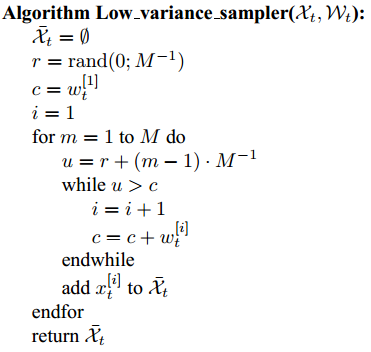
\includegraphics[scale=0.40]{images/low_variance_resampler}
\caption{Low variance re-sampler}
\label{fig:low_variance}
\end{figure}

Re-sampling happens after every 10th motion command. To get an estimate for the robots pose from all the particles, the particle with the highest weight is used. As a metric for the uncertainty of the estimate the variance of the particles is used.

\subsubsection{Explorer}
This class is used for calculating motion commands when the estimate uncertainty is high. It uses the lidar scan to look for obstacles and avoid them, while exploring as far away from its start position as possible. If nothing is in front of the robot, it will drive straight ahead. It looks at the measurements in front of the robot and if any of them are short it means an obstacle is ahead and it will do a 90 degree turn. It also looks for obstacles to the sides and turns to the free direction. If possible it will turn alternately 90 degrees left and right at each obstacle to avoid driving in circles. 

\subsubsection{PathFollower}
This class is used for calculating motion commands when the estimate uncertainty is low. It will use the AStarPlanner class to plan a path from the estimated position to a hard coded goal on the map. The path is a list of (x,y) points on the map. It will aim for the nearest point on the path and when it is close enough within some threshold it will start aiming for the next point.

\subsubsection{AStarPlanner}
This class implements the A* algorithm to do path planning. The different values of map are used as a cost-map to plan the best path.
